\documentclass[aspectratio=169]{beamer}

\usepackage[]{xcolor}
\usepackage{csquotes}
\usepackage{hyperref}
\usepackage{appendixnumberbeamer}

\usetheme{Dresden}
\usepackage[orientation=landscape,size=custom,width=16,height=9,scale=0.5,debug]{beamerposter}

\setbeamertemplate{navigation symbols}{}

\setbeamercolor{footline}{fg=blue}
\setbeamerfont{footline}{series=\bfseries}
\addtobeamertemplate{navigation symbols}{}{%
    \usebeamerfont{footline}%
    \usebeamercolor[fg]{footline}%
    \hspace{1em}%
    \insertframenumber
}



\title{Towards Formally Verified Rule Language Compilers}
\author{Antonio Hentschke}
\date{\today}


%\abstract{...}

\begin{document}

\begin{frame}
	\titlepage
\end{frame}



\section{Motivation}




\begin{frame}
	\frametitle{What is the problem}
	
	\begin{columns}
	\column{0.5\textwidth}
		\begin{itemize}
		\item optimisations need formal verification
			\begin{itemize}
			\item search for a fixpoint may not terminate, e.g. Skolem chase
			\item some algorithms optimize based on edge cases
			\end{itemize}
		\item correctness guarantees should not compromise efficiency
		\end{itemize}
	\column{0.5\textwidth}
		
	\end{columns}
	
\end{frame}



\begin{frame}
	\frametitle{Short trip to the world of compilers}
	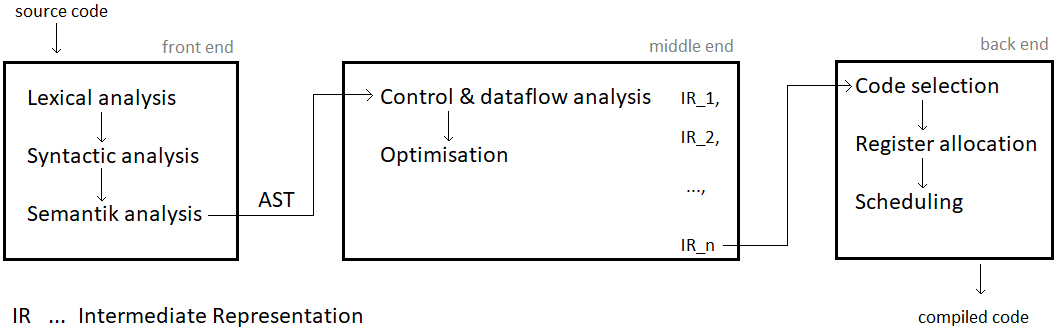
\includegraphics[scale=.5]{figures/compiler.png}
\end{frame}



\begin{frame}
	\frametitle{Formally verified compilers}
	\begin{itemize}
		\item 2 approaches
		\begin{itemize}
			\item internally verified - directly from scratch
			\item external verification aka. translation validation (more flexible)
		\end{itemize}
		
	\begin{center}
	\only<1>{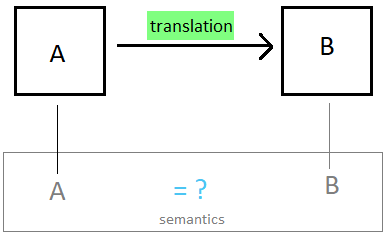
\includegraphics[scale=.4]{figures/fig2-tmp-a.png}}
	\only<2>{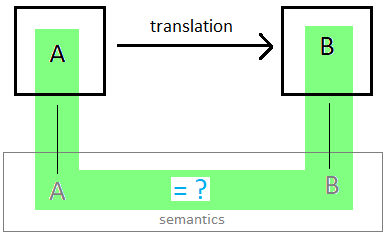
\includegraphics[scale=.4]{figures/fig2-tmp-b.png}}
	\end{center}
	
	
		\item formalize representations; formalize transitions; show preservation of \color{cyan} semantics
	\end{itemize}
\end{frame}



\begin{frame}
	\frametitle{Semantic preservation}
	\begin{itemize}
		\item formalize representations; formalize transitions; show preservation of semantics
		\item theorem provers like Coq or Lean can be used
	\end{itemize}
	\vspace{1em}
	\only<1>{ "If the compiler produces compiled code \(C\) from source code \(S\), without reporting compile-time errors, then every observable behavior (\(B\)) of \(C\) is either identical to an allowed behavior of \(S\), or improves over such an allowed behavior of \(S\) by replacing undefined behaviors with more defined behaviors." \small{[2]}}
	\only<2>{ \vspace{3em} \[ S \text{ \texttt{safe}} \Rightarrow \forall B, S \Downarrow B \iff C \Downarrow B \] }
	\only<3>{ \[ \forall S, C, Comp(S) = \text{\texttt{OK}} (C) \Rightarrow S \approx C \] }
\end{frame}



\begin{frame}
	\frametitle{Rule reasoning systems}
	
	\begin{columns}
	\column{0.6\textwidth}
	\only<1>{ \begin{enumerate}
		\item logic programming systems
		\item KG and deductive database engines
		\item specialised data-analytics systems
		\item data management frameworks
	\end{enumerate}}
	
	\only<2>{ \begin{enumerate}
		\item logic programming systems
		\item \textbf{KG and deductive database engines}
		\item \textbf{specialised data-analytics systems}
		\item data management frameworks
	\end{enumerate}}
	\vspace{1em}
	according to \textit{Nemo: Your Friendly and Versatile Rule Reasoning Toolkit} \small{[0]}
	

	\column{0.4\textwidth}
	
	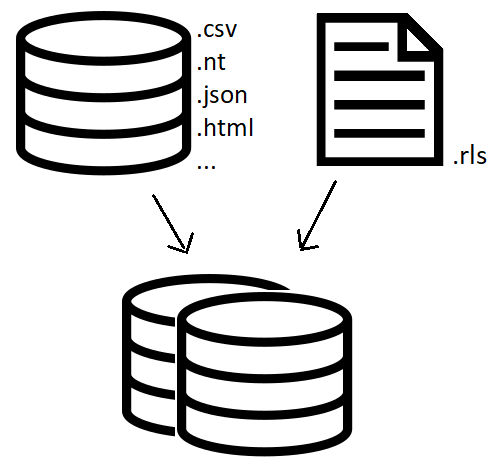
\includegraphics[scale=.3]{figures/fig1-tmp.png}
	\small{[1]}
	\end{columns}
\end{frame}



\section{Anatomy of Datalog Rule Engines}

\begin{frame}
	\frametitle{Nemo}
	\begin{center}
	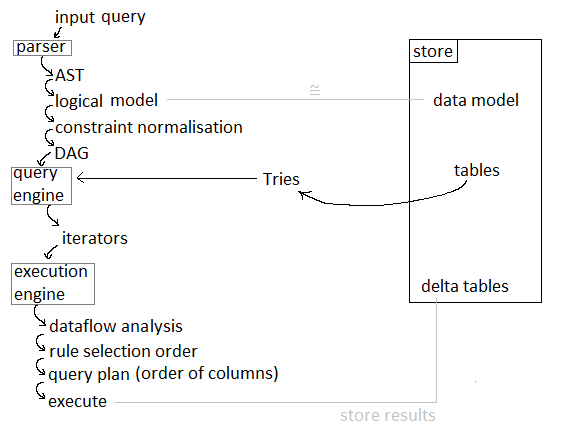
\includegraphics[scale=.5]{figures/nemo.png}
	\end{center}
	
\end{frame}

\begin{frame}
	\frametitle{VLog}
	\begin{center}
	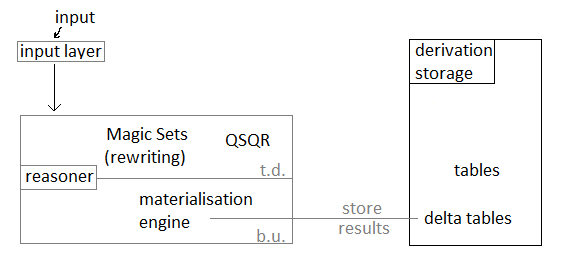
\includegraphics[scale=.6]{figures/vlog.png}
	\end{center}
\end{frame}

\begin{frame}
	\frametitle{Soufflé}
	\begin{center}
	
	\end{center}
\end{frame}

\begin{frame}
	\frametitle{Vadalog}
	\begin{center}
	
	\end{center}
\end{frame}

\begin{frame}
	\frametitle{LogicBlox}
	\begin{center}
	
	\end{center}
\end{frame}


\section{Task}

\begin{frame}
	\frametitle{What they have in common}
		todo
	
		\begin{tabular}{|c||c|c|c|c|c|} 
		 \hline
		  & nemo & VLog & Vadalog & LogicBlox & Soufflé \\
		 \hline\hline
		 type & 2, 3 & 2 & 2 & 3 & 3 \\ 
		 \hline
		 data strct & tries & QSQR & ? & treaps & tries \\
		 \hline
		 graph repr & DAG & magic sets & KG & ? & B-tree \\
		 \hline
		 storage & delta tables & derivation storage & KG repos & workspaces & R.A.M \\
		 \hline
		 join & LFTJ & ? & ? & LFTJ & loop-based \\
		 \hline
		 reasoning & t.d. & t.d./b.u. & . & . & . \\
		 \hline
		\end{tabular}
		
		\vspace{1em}
		t.d. = top-down (query-driven reasoning)
		
		b.u. = bottom-up (materialisation)

\end{frame}

\begin{frame}
	\frametitle{Concrete plans for verification}
	todo
	\begin{itemize}
		\item semi-naive evaluation (since it's optimized)
		\item LFTJ (since it's optimized)
		\item 1-parallel restricted chase
		\item (skolem chase)
	\end{itemize}
\end{frame}

\begin{frame}
	\frametitle{References}
	\tiny{
	[0] \textbf{classification of rule reasoning systems} from \textit{Nemo: Your Friendly and Versatile Rule Reasoning Toolkit}, Alex Ivliev and Lukas Gerlach and Simon Meusel and Jakob Steinberg and Markus Krötzsch, \url{https://iccl.inf.tu-dresden.de/w/images/f/fb/KR-2024-CR.pdf}
	
	[1] \textbf{database icon} \url{https://linearicons.com/}, created by \url{https://perxis.com/} - \url{https://cdn.linearicons.com/free/1.0.0/Linearicons-Free-v1.0.0.zip}, CC BY-SA 4.0, \url{https://commons.wikimedia.org/w/index.php?curid=77236210};
	
	\textbf{note icon} SimpleIcon \url{http://www.simpleicon.com/}, CC BY 3.0 \url{https://creativecommons.org/licenses/by/3.0}, via Wikimedia Commons; changes were made to the graphics
	
	[2] \textbf{definition of semantic preservation} taken from \textit{CompCert - A Formally Verified Optimizing Compiler}, Leroy, Xavier and Blazy, Sandrine and Kästner, Daniel and Schommer, Bernhard and Pister, Markus and Ferdinand, Christian, \url{https://inria.hal.science/hal-01238879/file/erts2016_compcert.pdf}}
  
\end{frame}


	
\end{document}